\PassOptionsToPackage{sols}{handout}
\documentclass[main]{subfiles}
\setcounterrefbeforedot{chapter}{m-ws5-1}
\setcounterrefafterdot{section}{m-ws5-1}
\addtocounter{section}{-1}
\usepackage{solutions}

\begin{document}

\ifSubfilesClassLoaded{%
  \chaptermark{\chapterfive}
}{}

\section{Net Change} \label{ws5-1}

\begin{problemonly}
    \begin{framed}

\textbf{Key Ideas}:

\begin{itemize}[topsep=0pt,partopsep=0pt,parsep=8pt,itemsep=0pt]

\item You should understand what we mean by net change.  For example,
  ``the net change in price of apples from $t = 1$ to $t = 5$'' is
  simply equal to ``(price of apples at time $t = 5$) minus (price of
  apples at time $t = 1$).''

\item Given a graph, table of values, or formula for a rate function,
  you should be able to \emph{approximate} net change using left-hand
  and right-hand sums.  (Throughout this unit, it will be important to
  distinguish between when you are making an approximation and when you
  are finding an exact answer.)  You should be comfortable with the
  notation $L_n$ and $R_n$ that we use for these sums.

\item You should understand the notion of ``signed area'' and be able to
  visualize net change as signed area under a rate curve.

\end{itemize}
\end{framed}
\end{problemonly}

\begin{enumerate}
\item 
  \note{If you would like to use the Riemann Sums applet with this, you can enter the function as \begin{mathematica} If[x < 2, 7, (x - 4)^2 + 3]\end{mathematica}}


    On Patriot's Day last year, Deb ran the Boston Marathon.  For the
    first two hours, Deb ran at a constant speed of 7 mph.  For the next
    two hours, Deb's speed in miles per hour was given by 
    $v(t) = (t - 4)^2 + 3$, where 
    $t$ was hours after she started the race.

    Deb's 12-year-old brother would like to use this information to
    figure out how far Deb ran in the first 4 hours of the race.  How
    could he \textit{approximate} this distance?  (He's only 12, so he
    doesn't know any calculus!)

    \begin{enumerate}
    \begin{minipage}{0.57\textwidth} \vspace{-64pt}
    \item He starts by looking at the first 2 hours and draws
        the graph shown to the right.
        \begin{enumerate}[left=-6pt]
          \item
            How far did Deb run in the first 2 hours of the race?
          \item Represent the distance Deb ran as an area on the graph.
          \item Why is this distance being represented as an
            area on this particular graph, rather than being represented
            as a length?
        \end{enumerate}
    \end{minipage}
    \begin{minipage}{0.35\textwidth} \vspace{-8pt}
    \begin{center}
        \begin{tikzpicture}
            \begin{axis}[
                xlabel = $t$ (hr),
                ylabel = speed (mph),
                xmin = -0.25, xmax = 4.25,
                ymin = -0.25, ymax = 8.75,
                grid = both,
                xtick = {0,1,2,3,4},
                ytick = {0,2,4,6,8},
                minor y tick num = 1,
                minor x tick num = 0,
                width = 3.5in,
                axis equal image,
            ]
            \addplot[name path=f,ultra thick,black,domain=0:2]{7};
            \addplot[draw=none,name path=g]{0};
            \solonly{
            \addplot[fill=green, opacity=0.5] fill between[of=f and g, 
            soft clip={domain=0:2}];
            }
            \end{axis}
        \end{tikzpicture}
    \end{center}
    \end{minipage}
    
    \pspace{\vfill}

    \begin{solution}
    We can find Deb's \emph{exact} distance during the first 2 hours
    easily: Deb runs at a constant speed of 7 miles/hour, so she runs a
    total distance of (7 miles/hour)(2 hours) = 14 miles.  We can
    visualize this as the area of a rectangle on the graph of Deb's speed.
    
    On the graph, this distance is represented as an area and not a length 
    because the horizontal axis has units of hours and the vertical axis has
    units of miles/hour, so an area on the graph has units of 
    $\text{hours} \times \frac{\text{miles}}{\text{hours}} = \text{miles}$.
    \end{solution}

  \item He then tackles the second two hours, 
    from $t=2$ to $t=4$. He knows ``distance = speed $\times$ time,''
    but this only works if the speed is constant.
    
    \begin{minipage}{0.57\textwidth}\vspace{-80pt}
      \begin{enumerate}[left=-6pt]

      \item
      How can he approximate the distance Deb ran?

      \item How could you represent this approximation
      on the graph?

      \item Can you determine whether this approximation
      underestimates Deb's distance or overestimates it?

      \item How can this approximation be improved upon?
      
      \end{enumerate}
    \end{minipage}
    \begin{minipage}{0.35\textwidth} \vspace{-8pt}
    \begin{center}
        \begin{tikzpicture}
            \begin{axis}[
                xlabel = $t$ (hr),
                ylabel = speed (mph),
                xmin = -0.25, xmax = 4.25,
                ymin = -0.25, ymax = 8.75,
                grid = both,
                xtick = {0,1,2,3,4},
                ytick = {0,2,4,6,8},
                minor y tick num = 1,
                minor x tick num = 0,
                width = 3.5in,
                axis equal image,
            ]
            \addplot[ultra thick,black,domain=0:2,name path = f]{7};
            \addplot[ultra thick,black, domain=2:4,name path = g]{(x-4)^2+3};
            \addplot[draw=none,name path=h]{0};
            \solonly{
            \addplot[fill=green, opacity=0.5] fill between[of=f and h,
            soft clip={domain=0:2}];
            \addplot[fill=green, opacity=0.5] fill between[of=g and h,
            soft clip={domain=2:4}];
            }
            \end{axis}
        \end{tikzpicture}
    \end{center}
    \end{minipage}
    \end{enumerate}
    \pspace{\vfill}

  
  \begin{solution}
    For the next 2 hours, Deb's speed is no longer constant, so we can
    only approximate her distance.  There are lots of possible methods,
    but the one we settled on in class was using a left- or right-hand
    sum.  The basic idea of each is to \emph{pretend}, as an
    approximation, that Deb runs at a constant speed on shorter intervals
    of time.  Here, we'll do one example of each:
    \begin{itemize}
    \item \emph{A left-hand sum with 2 sub-intervals}

      Here, we break the 2 hour period into two 1-hour chunks and pretend
      that Deb's speed for the entire hour-long chunk is whatever it was
      at the start of the chunk:
      \begin{itemize}
      \item The first chunk (really the 3rd hour of running): Deb's speed
        at the start of the 3rd hour was $v(2) = 7$ mph, so we'll just
        pretend that she ran at 7 mph for the entire hour.  If this was
        the case, she'd have run (7 mph)(1 hour) = 7 miles in the 3rd
        hour.  (Note that this is an overestimate of Deb's distance
        because she was slowing down for the whole hour.) 
      \item The second chunk (really the 4th hour of running): Deb's speed
        at the start of the 4th hour was $v(3) = 4$ mph, so we'll just
        pretend thats he ran at 4 mph for the entire hour.  If this was the
        case, she'd have run (4 mph)(1 hour) = 4 miles in the 4th hour.
        (Again, this is an overestimate of Deb's distance because she was
        slowing down for the whole hour.)
      \end{itemize}
      So, one estimate for Deb's distance over the last 2 hours is 7 miles
      + 4 miles = 11 miles, and this is an overestimate.  We can picture
      this estimate as the area in the following 2 rectangles:
      \begin{center}
        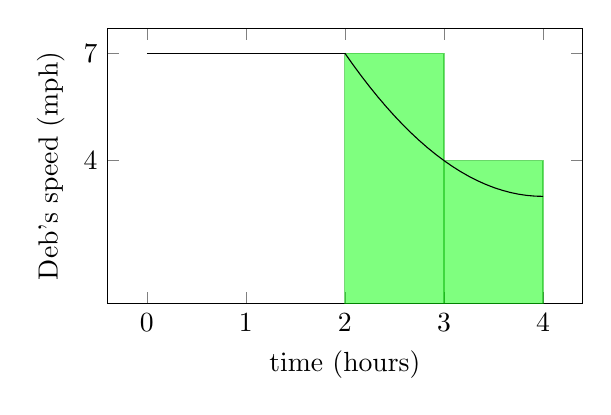
\begin{tikzpicture}
          \begin{axis}[xlabel=time (hours), ylabel=Deb's speed (mph), cycle
            list=black, ymin=0, ytick={4, 7}, width=3in, height=2in] 
            \addplot+[ybar interval, fill=green, opacity=0.5,
            draw=green!70!black] coordinates 
            {
              (2, 7)
              (3, 4)
              (4, 4)
            };        
            \addplot+[domain=0:2] {7};
            \addplot+[domain=2:4] {(x-4)^2+3};
          \end{axis}
        \end{tikzpicture}
      \end{center}      

    \item \emph{A right-hand sum with 4 sub-intervals}

      Using 4 sub-intervals means that we break the 2 hour period into
      four chunks (each 30 minutes long).  Doing a right-hand sum means
      that we pretend that Deb's speed for the entire 30-minute chunk is
      whatever it was at the \emph{end} of the chunk:
      \begin{itemize}
      \item For the first chunk (between time $t = 2$ and $t = 2.5$), we
        pretend that Deb's speed was $v(2.5) = 5.25$ mph for the entire 30
        minutes.  If this was the case, she'd have run (5.25 mph)(0.5
        hours) = 2.625 miles over this 30 minutes.  (Note that this is an
        underestimate of Deb's distance because she was slowing down, and
        $5.25$ was her lowest speed during this half hour.)
      \item For the second chunk (between $t = 2.5$ and $t = 3$), we
        pretend that Deb's speed was $v(3) = 4$ mph for the entire 30
        minutes.  If this was the case, she'd have run (4 mph)(0.5 hours) =
        2 miles over this 30 minutes.
      \item For the third chunk (between $t = 3$ and $t = 3.5$), we
        pretend that Deb's speed was $v(3.5) = 3.25$ mph for the entire 30
        minutes.  If this was the case, she'd have run (3.25 mph)(0.5
        hours) = 1.625 miles.
      \item For the fourth chunk (between $t = 3.5$ and $t = 4$), we
        pretend that Deb's speed was $v(4) = 3$ mph for the entire 30
        minutes.  If this was the case, she'd have run (3 mph)(0.5 hours) =
        1.5 miles.
      \end{itemize}
      Thus, our total estimate for Deb's distance over the last 2 hours is
      $2.625 + 2 + 1.625 + 1.5 = 7.75$ miles, and this is an
      underestimate.  We can picture this estimate as the area in the
      following 4 rectangles:
      \begin{center}
        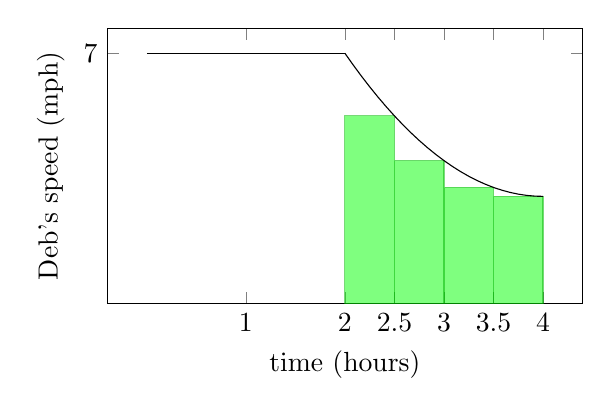
\begin{tikzpicture}
          \begin{axis}[xlabel=time (hours), ylabel=Deb's speed (mph), cycle
            list=black, ymin=0, ytick={7}, xtick={1, 2, 2.5, 3, 3.5, 4},
            width=3in, height=2in] 
            \addplot+[ybar interval, fill=green, opacity=0.5,
            draw=green!70!black] coordinates 
            {
              (2, 5.25)
              (2.5, 4)
              (3, 3.25)
              (3.5, 3)
              (4, 3)
            };        
            \addplot+[domain=0:2] {7};
            \addplot+[domain=2:4] {(x-4)^2+3};
          \end{axis}
        \end{tikzpicture}
      \end{center}      

    \end{itemize}

    A couple of notes:
    \begin{itemize}
    \item If we put our two estimates together, we get slightly more
      definitive information: Deb's total distance over the 4 hours was
      between $14 + 7.75 = 21.75$ miles and $14 + 11 = 25$ miles.  (Her
      actual distance turns out to be $\frac{68}{3} = 22.666\ldots$ miles,
      and one of our goals in the next few weeks is to see how to arrive
      at this exact answer!)

    \item To get more accurate approximations, we should use more
      sub-intervals.  To get an exact approximation, we should take the
      limit as the number of sub-intervals $\to \infty$; this can be
      visualized as the exact area under his velocity curve from $t = 0$
      to $t = 4$:
      \begin{center}
        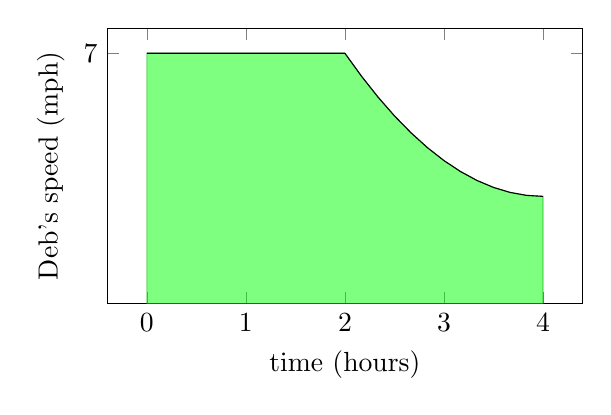
\begin{tikzpicture}[declare function={
            f(\x) = (\x <= 2) * 7 + (\x > 2) * ((\x - 4)^2 + 3);
          }]          
          \begin{axis}[xlabel=time (hours), ylabel=Deb's speed (mph), cycle
            list=black, ymin=0, ytick={7}, width=3in, height=2in] 
            \addplot+[fill=green, opacity=0.5,
            draw=green!70!black, domain=0:4] {f(x)} \closedcycle;
            \addplot+[domain=0:4, black] {f(x)};
          \end{axis}
        \end{tikzpicture}
      \end{center}
    \end{itemize}
  \end{solution}

\item 
    Last year, Deb's friend Andrea also ran the Boston Marathon.  For the
    first two hours, Andrea ran together with Deb (at a constant speed of
    7 mph).  For the next two hours, Andrea's speed was given by $v(t) =
    11 - 2t$, where $t$ was hours after she started the race. 
    \begin{enumerate}[topsep=0pt]

    \begin{minipage}{0.57\textwidth} \vspace{-64pt}
    \item Sketch the graph of Andrea's velocity over the graph of Deb's.
        \begin{enumerate}[left=-6pt]
            \item How far did
            Andrea run in the first 4 hours?  Is your answer an
            approximation, or
            is it exact? If it's an approximation, how can you make 
            it better?
            (A graph may help you.)
          \item
            Who was ahead after 4 hours?
          \item Challenge: Color the area that corresponds to the lead
            of the faster woman.
        \end{enumerate}
    \end{minipage}
    \begin{minipage}{0.35\textwidth} \vspace{-8pt}
    \begin{center}
        \begin{tikzpicture}
            \begin{axis}[
                xlabel = $t$ (hr),
                ylabel = speed (mph),
                xmin = -0.25, xmax = 4.25,
                ymin = -0.25, ymax = 8.75,
                grid = both,
                xtick = {0,1,2,3,4},
                ytick = {0,2,4,6,8},
                minor y tick num = 1,
                minor x tick num = 0,
                width = 3.5in,
                axis equal image,
            ]
            \addplot[ultra thick,dashed,black,domain=0:2,name path=a]{7};
            \addplot[ultra thick,dashed,black,domain=2:4,name path=g]
            {(x-4)^2+3};
            \solonly{
            \addplot[ultra thick, domain=0:2]{7};
            \addplot[ultra thick,domain=2:4,name path=f]{11-2*x};
            \addplot[draw=none,name path=b]{0};
            \addplot[fill=green,opacity=0.5] fill between[of=f and g, soft clip={domain=2:4}];
            \addplot[fill=green!70!black,opacity=0.5] 
            fill between[of=a and b, soft clip={domain=0:2}];
            \addplot[fill=green!70!black,opacity=0.5]
            fill between[of=g and b, soft clip={domain=2:4}];
            }
            \end{axis}
        \end{tikzpicture}
    \end{center}
    \end{minipage}
    \end{enumerate}

  \pspace{\stretch{1}}

  \begin{solution}
    We can visualize Andrea's exact distance in the first 4 hours as the
    area under her velocity graph between $t = 0$ and $t = 4$:
    \begin{center}
      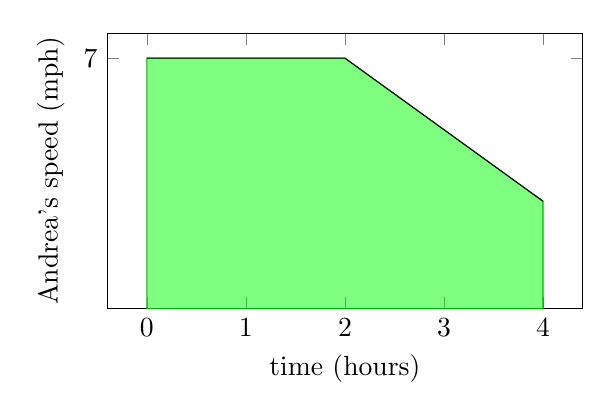
\begin{tikzpicture}[declare function={ 
          f(\x) = (\x < 2) * (7) + (\x >= 2) * (11-2*\x); 
        }] 
        \begin{axis}[cycle list=black, xlabel=time (hours),
          ylabel=Andrea's speed (mph), ymin=0, ytick={7}, width=3in,
          height=2in]  
          \addplot+[domain=0:4, fill=green, fill opacity=0.5, draw=green!70!black] {f(x)} \closedcycle; 
          \addplot+[domain=0:4] {f(x)}; 
        \end{axis} 
      \end{tikzpicture}      
    \end{center}
    We can find this area exactly using geometry, by splitting the region
    into rectangles and a triangle.  First, note that $v(4) = 3$.
    \begin{center}
      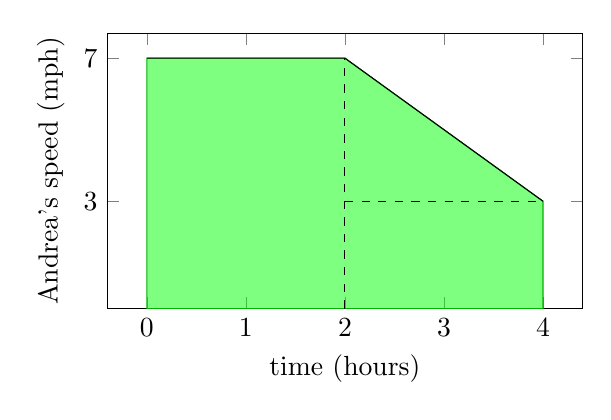
\begin{tikzpicture}[declare function={ 
          f(\x) = (\x < 2) * (7) + (\x >= 2) * (11-2*\x); 
        }] 
        \begin{axis}[cycle list=black, xlabel=time (hours),
          ylabel=Andrea's speed (mph), ymin=0, ytick={3, 7}, width=3in,
          height=2in]  
          \addplot+[domain=0:4, fill=green, fill opacity=0.5, draw=green!70!black] {f(x)} \closedcycle; 
          \addplot+[domain=0:4] {f(x)};
          \draw[dashed] (axis cs: 2, 0) -- (axis cs: 2, 7);
          \draw[dashed] (axis cs: 2, 3) -- (axis cs: 4, 3);
        \end{axis} 
      \end{tikzpicture}      
    \end{center}
    The left rectangle has area $7 \cdot 2 = 14$, the right rectangle has
    area $3 \cdot 2 = 6$, and the triangle has area $\frac{1}{2} \cdot 4
    \cdot 2 = 4$, so the total area is $24$.  Thus, Andrea ran
    \fbox{exactly 24 miles} in the first 4 hours.

    After 4 hours, Andrea was ahead of Deb. This because they ran at the same
    speed for the first two hours, and in the next two hours, Andrea's
    speed was always higher than Deb's. The area that corresponds to the
    Andrea's lead is the area between the graph of Andrea's speed and the
    graph of Deb's speed.
  \end{solution}

\pspace{\newpage}

\item 
  \note{This is to introduce the idea of \textit{signed} area.}

  Fresh Pond is a reservoir about 2 miles from Harvard, which holds
  drinking water for the city of Cambridge.  The amount of water in the
  pond changes over time due to rainfall and water being pumped in and out
  of the reservoir.  Suppose that the following graph shows the
  \textit{rate} at which water is entering or leaving the reservoir
  (measured in millions of gallons per day) at time $t$, where $t$ is
  measured in days.  

  {
    \providecommand{\graphcommand}[1]{}
    \renewcommand{\graphcommand}[1]{
      \begin{tikzpicture}[declare function={
          f(\x) = and(0 <= \x, \x <=2) * (+-0.16649377593360995*\x^3+-7.718257261410789e-61*\x^2+-0.8340248962655602*\x^1+18*\x^0)
          + and(2 < \x, \x <=3) * (+-1.1690871369294606*\x^3+6.015560165975104*\x^2+-12.865145228215768*\x^1+26.020746887966805*\x^0)
          + and(3 < \x, \x <=4) * (+2.8433609958506225*\x^3+-30.096473029045644*\x^2+95.47095435684648*\x^1+-82.31535269709543*\x^0)
          + and(4 < \x, \x <=6) * (+-0.5570539419087137*\x^3+10.70850622406639*\x^2+-67.74896265560166*\x^1+135.31120331950208*\x^0)
          + and(6 < \x, \x <=8) * (+-0.11358921161825726*\x^3+2.7261410788381744*\x^2+-19.854771784232366*\x^1+39.522821576763484*\x^0)
          ;}]
        \begin{axis}[cycle list=black, 
          grid=major, 
          xmin = -0.25, xmax = 8.25, ymin = -9.25, ymax = 18.25,
          xtick={0, 1, ..., 8},
          ytick={-9,-6, ..., 18}, 
          xlabel=$t$, enlarge y limits=0.01, 
          axis line style={shorten >=-8pt, shorten <=-8pt}, 
          xlabel style={xshift=8pt}]
          % generated using 
          % https://tools.timodenk.com/cubic-spline-interpolation
            \addplot[domain=0:8] {f(x)};
            #1
        \end{axis}
      \end{tikzpicture}
    }
    \newsavebox{\graph}
    \savebox{\graph}{
      \graphcommand{}
    }

    \begin{enumerate}
    \item
      \begin{problem}
        How could you \textit{approximate} the net change in the amount of
        water in Fresh Pond between $t = 0$ and $t = 8$?
        How can you visualize your approximation on the graph?
      \end{problem}

      \begin{tabular}{c}
        {\small rate of change of amount of water in Fresh Pond} \\
        {\small (millions of gallons / day)} \\
        \usebox{\graph}
      \end{tabular}

      \begin{solution}
        We could again use a left- or right-hand sum; the main new issue
        in this problem is that sometimes the rate is negative.  This
        happens when the pond is losing water; for example, if we call the
        rate function $r(t)$, the fact that $r(6) = -6$ means that, at $t
        = 6$, the pond is losing water at an instantaneous rate of 6
        million gallons per day.  So, for instance, it would be reasonable
        to approximate the net change in the amount of water between $t =
        6$ and $t = 7$ as $(-6 \text{ million gallons/day})(1 \text{
          day}) = -6$ million gallons, with the negative sign
        indicating that there was a net loss of water in that time.
        Graphically, we could represent this as the negative of the area
        of the rectangle below:
        \begin{center}
          \graphcommand{
            \addplot+[ybar interval, fill=red, opacity=0.5,
            draw=red!70!black] coordinates 
            {
              (6, -6)
              (7, -6)
            };
          }
        \end{center}
        If we did the same thing for all $8$ one-day interval between $t =
        0$ and $t = 8$, we'd end up adding the areas of the green
        rectangles and subtracting the areas of the red rectangles:
        \begin{center}
          \graphcommand{
            \addplot+[ybar interval, fill=green, opacity=0.5,
            draw=green!70!black] coordinates 
            {
              (0, {f(0)}) (1, {f(1)}) (2, {f(2)}) (3, {f(3)}) (4, {f(4)}) 
            };
            \addplot+[ybar interval, fill=red, opacity=0.5,
            draw=red!70!black] coordinates 
            {
              (4, {f(4)}) (5, {f(5)}) (6, {f(6)}) (7, {f(7)}) (8, {f(8)}) 
            };
          }
        \end{center}

      \end{solution}      

    \item
    \begin{problem}[\vfill]
        How could you get a \emph{better} approximation? And an
        even better one? How can you visualize these on the graph?
    \end{problem}

    \begin{solution}
    We could get a better approximation by partitioning the interval into between $t = 0$ and $t = 8$ into $16$ half-day sub-intervals:
        \begin{center}
          \graphcommand{
            \addplot+[ybar interval, fill=green, opacity=0.5,
            draw=green!70!black] coordinates 
            {
              (0, {f(0)}) (0.5, {f(0.5)}) (1, {f(1)}) (1.5, {f(1.5)}) (2, {f(2)}) (2.5, {f(2.5)}) (3, {f(3)}) (3.5, {f(3.5)}) (4, {f(4)}) 
            };
            \addplot+[ybar interval, fill=red, opacity=0.5,
            draw=red!70!black] coordinates 
            {
              (4, {f(4)}) (4.5, {f(4.5)}) (5, {f(5)}) (5.5, {f(5.5)}) (6, {f(6)}) (6.5, {f(6.5)}) (7, {f(7)}) (7.5, {f(7.5)}) (8, {f(8)}) 
            };
          }
        \end{center}
        We could keep making the subintervals smaller and smaller to get
        better approximations, and the rectangles would get progressively
        thinner.
      \end{solution}  

    

    \item
      \begin{problem}[\vfill]
        How could you visualize the \textit{exact} net change in the amount
        of water in Fresh Pond between $t = 0$ and $t = 8$?
      \end{problem}

    \begin{solution}
      In {{{{\#3}}(a)}}, we figured out how to
      approximate this net change.  To get a better approximation, we
      should use more time intervals, with each being shorter (as opposed
      to what we did, which was to use 16 half-day long intervals in our
      last picture).  To get the exact net change, we'd want to take the
      limit as the number of sub-intervals $\to \infty$; we can visualize
      this as the \emph{signed area} between the curve and the $x$-axis,
      where the area is positive when the curve is above the $x$-axis and
      negative when the curve is below the $x$-axis.  That is, it's the
      area of the green region minus the area of the red region:
      \begin{center}
        \graphcommand{%
          \addplot+[domain=0:4, fill=green, fill opacity=0.5,
          draw=green!70!black] { f(x) } 
          \closedcycle;
          \addplot+[domain=4:8, fill=red, fill opacity=0.5,
          draw=red!70!black] {f(x)} 
          \closedcycle; 
        }
      \end{center}
    \end{solution}

    \item
      \begin{problem}[\vfill]
        Does the pond have more water at time $t = 0$ or time $t = 8$?
      \end{problem}

      \begin{solution}
        From our picture in {{{{\#3}}(b)}}, we
        can see that the net change in the amount of water between $t = 0$
        and $t = 8$ is positive because the green region is larger than
        the red one.  Saying that the net change between $t = 0$ and $t =
        8$ is positive exactly means that the pond has more water at
        \fbox{$t = 8$} than at $t = 0$.
      \end{solution}

    \item
      \begin{problem}[\vfill\newpage]
        Does the pond have more water at time $t = 3$ or time $t = 8$?
      \end{problem}

      \begin{solution}
        Now, it's more useful to visualize the net change between $t = 3$
        and $t = 6$; that's the signed area under the curve\footnote{Even
          though people usually say ``signed area under the curve'', it's
          really more accurate to say ``signed area between the curve and
          the $x$-axis''.} between $t = 3$ and $t = 6$:
        \begin{center}
          \graphcommand{%
            \addplot+[domain=3:4, fill=green, fill opacity=0.5,
            draw=green!70!black] { f(x) } 
            \closedcycle;
            \addplot+[domain=4:6, fill=red, fill opacity=0.5,
            draw=red!70!black] {f(x)} 
            \closedcycle;
            \addplot+[domain=0:8] {f(x)};
          }
        \end{center}
        This signed area is negative, so there is a net loss in water from
        $t = 3$ to $t = 6$; therefore, there is more water in the pond at
        \fbox{$t = 3$} than at $t = 6$. 
      \end{solution}

    \item
      \begin{problem}[\vfill]
        Use a left-hand sum with 4 subintervals to approximate the net
        change in the amount of water between $t = 0$ and $t = 8$.  (We
        often use the notation $L_4$ for ``left-hand sum with 4
        subintervals.'') Represent this on the graph on the left.

        Then, use a right-hand sum with 4 subintervals (we'll typically use
        the notation $R_4$ for this). Repreesnt this on the graph
        on the right.

          \begin{tabular}{c c c}
            \scalebox{0.75}{\usebox{\graph}} &
            \hspace{0.5in} &
            \scalebox{0.75}{\usebox{\graph}}
          \end{tabular}
      \end{problem}

      \begin{solution}
        We can visualize $L_4$ and $R_4$ as signed areas of rectangles:
        \begin{center}
          \begin{tabular}{c c c}
            \scalebox{0.75}{\graphcommand{
                \addplot+[ybar interval, fill=green, opacity=0.5,
                draw=green!70!black] coordinates 
                {
                  (0, {f(0)}) (2, {f(2)}) (4, {f(4)}) 
                };
                \addplot+[ybar interval, fill=red, opacity=0.5,
                draw=red!70!black] coordinates 
                {
                  (4, {f(4)}) (6, {f(6)}) (8, {f(8)}) 
                };
              }} &
            \hspace{0.5in} &
            \scalebox{0.75}{\graphcommand{
                \addplot+[ybar interval, fill=green, opacity=0.5,
                draw=green!70!black] coordinates 
                {
                  (0, {f(2)}) (2, {f(4)}) (4, {f(4)}) 
                };
                \addplot+[ybar interval, fill=red, opacity=0.5,
                draw=red!70!black] coordinates 
                {
                  (4, {f(6)}) (6, {f(8)}) (8, {f(8)}) 
                };
              }} \\
            $L_4$ && $R_4$
          \end{tabular} 
        \end{center}
        From the pictures, we can see that
        \begin{align*}
          L_4 &= f(0) \cdot 2 + f(2) \cdot 2 + f(4) \cdot 2 + f(6) \cdot 2
          \\
          &= 18 \cdot 2 + 15 \cdot 2 + 0 \cdot 2 + (-6) \cdot 2 \\
          &= 54 \\
          R_4 &= f(2) \cdot 2 + f(4) \cdot 2 + f(6) \cdot 2 + f(8) \cdot 2
          \\
          &= 15 \cdot 2 + 0 \cdot 2 + (-6) \cdot 2 + (-3) \cdot 2 \\
          &= 12 
        \end{align*}
      \end{solution}

    \end{enumerate}

  }

\pspace{\vfill}

\item 
  \begin{problem}
    Arctic sea ice grows in the Arctic winter and melts in the Arctic
    summer. The following is a model\footnote{While the model is
      hypothetical, it is loosely based on data found at the National Snow
      and Ice Data Center website
      \url{http://nsidc.org/arcticWS21_fig1_seaicenews/2008}.}  of the
    rate of growth and melt of Arctic Sea ice, $r(t)$, from Sept 2007 $(t=
    0$) to Sept 2008 $(t=12)$. The rate is measured in millions of square
    kilometers per month.  What is the net change in Arctic sea ice
    between September 2007 and September 2008?
  \end{problem}

  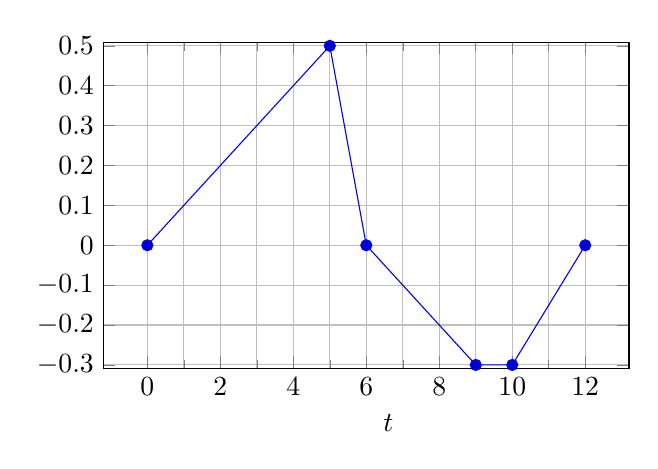
\begin{tikzpicture}
    \begin{axis}[minor xtick={1, 3, ..., 11}, ytick={-0.3, -0.2, ...,
        0.51}, grid=both, enlarge y limits=0.01, tick label
      style={/pgf/number format/fixed}, xlabel=$t$, axis line
      style={shorten >=-8pt, shorten <=-8pt}, xlabel
      style={xshift=8pt}, width=3.25in, height=2.25in ]
      \addplot+[sharp plot] coordinates
      {
        (0, 0)
        (5, 0.5)
        (6, 0)
        (9, -0.3)
        (10, -0.3)
        (12, 0)
      };
    \end{axis}
  \end{tikzpicture}

  \pspace{\vfill}

  \begin{solution}
    The net change in Arctic sea ice between September 2007 and September
    2008 can be pictures as the signed area under $r(t)$ from $t = 0$ to
    $t = 12$:
    \begin{center}
      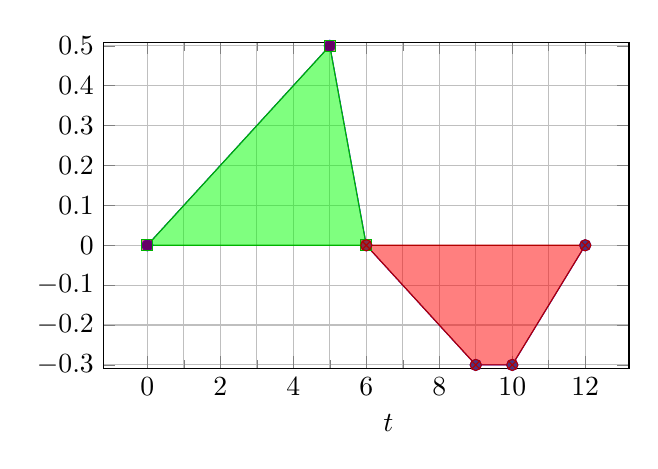
\begin{tikzpicture}
        \begin{axis}[minor xtick={1, 3, ..., 11}, ytick={-0.3, -0.2, ...,
            0.51}, grid=both, enlarge y limits=0.01, tick label
          style={/pgf/number format/fixed}, xlabel=$t$, axis line
          style={shorten >=-8pt, shorten <=-8pt}, xlabel
          style={xshift=8pt}, width=3.25in, height=2.25in ]
          \addplot+[sharp plot] coordinates
          {
            (0, 0)
            (5, 0.5)
            (6, 0)
            (9, -0.3)
            (10, -0.3)
            (12, 0)
          };
          \addplot+[sharp plot, fill=green, fill opacity=0.5,
          draw=green!70!black] coordinates 
          {
            (0, 0)
            (5, 0.5)
            (6, 0)
          } \closedcycle;
          \addplot+[sharp plot, fill=red, fill opacity=0.5,
          draw=red!70!black] coordinates
          {
            (6, 0)
            (9, -0.3)
            (10, -0.3)
            (12, 0)
          } \closedcycle;
        \end{axis}
      \end{tikzpicture}
    \end{center}
    The green region is a triangle of width 6 and height 0.5, so it has
    area $\frac{1}{2} (6)(0.5) = 1.5$.  The red region can be broken up
    into a triangle (from $t = 6$ to $t = 9$), a rectangle (from $t = 9$
    to $t = 10$), and a triangle (from $t = 10$ to $t = 12$), and its
    total area is $1.05$.  So, the overall signed area from $t = 0$ to $t
    = 12$ is $1.5 - 1.05 = 0.45$.  Therefore, over the year, the Arctic
    experiences a net increase of $0.45$ square kilometers of sea ice.
  \end{solution}

\pspace{\vfill}

\end{enumerate}


\end{document}